% =====================================================================
%  Oil Price Shocks and India's Terms of Trade: An Empirical Assessment
%  International Economics, group presentation (15 min + 15 min viva)
%
%  Compile with pdfLaTeX (Overleaf default) or:  latexmk -pdf slides.tex
%  Speaker-notes version:  latexmk -pdf -jobname=slides_with_notes \
%                            -usepretex='\def\withnotes{}' slides.tex
%  (On Overleaf: uncomment the \def\withnotes line below instead.)
%
%  Figures in figures/ and tables in tables/ are produced by
%  src/slide_figures.py from the project's outputs. Do not edit numbers
%  by hand here: change the analysis and regenerate.
% =====================================================================
% \def\withnotes{}   % <- uncomment on Overleaf to get the notes version
\documentclass[aspectratio=169,11pt]{beamer}

\usetheme[progressbar=frametitle, numbering=fraction, block=fill]{metropolis}
\usepackage[T1]{fontenc}
\usepackage[sfdefault,scaled=.95]{FiraSans}
\usepackage{FiraMono}
\usepackage{amsmath}
\usepackage{booktabs}
\usepackage{graphicx}
\usepackage[most]{tcolorbox}
\usepackage{tikz}
\usepackage{appendixnumberbeamer}

% Notes version: every slide is followed by a page with a thumbnail of it and the speaker script.
\ifdefined\withnotes
  \setbeameroption{show notes}
  \setbeamertemplate{note page}{%
    \vspace{5mm}\noindent\hspace*{6mm}%
    \begin{minipage}[t]{.37\paperwidth}\vspace{0pt}\fbox{\insertslideintonotes{0.35}}\end{minipage}%
    \hspace{4mm}%
    \begin{minipage}[t]{.5\paperwidth}\vspace{0pt}\raggedright\footnotesize\insertnote\end{minipage}}
\fi

% characters that pdfLaTeX does not know by default
\DeclareUnicodeCharacter{2212}{\ensuremath{-}}
\DeclareUnicodeCharacter{2192}{\ensuremath{\rightarrow}}

% ---------------------------------------------------------------- colours
\definecolor{navy}{HTML}{0F1B2D}
\definecolor{oil}{HTML}{EB6834}     % orange: terms of trade, highlights
\definecolor{sea}{HTML}{2A78D6}     % blue: oil price
\definecolor{card}{HTML}{F2F4F7}
\definecolor{cardwarm}{HTML}{FDEDE6}
\definecolor{muted}{HTML}{6B6A66}
\definecolor{ink}{HTML}{1A1A1A}

\setbeamercolor{frametitle}{bg=navy, fg=white}
\setbeamercolor{progress bar}{fg=oil, bg=navy!25}
\setbeamercolor{title separator}{fg=oil}
\setbeamercolor{alerted text}{fg=oil}
\setbeamercolor{normal text}{fg=ink, bg=white}
\setbeamercolor{background canvas}{bg=white}
\setbeamercolor{block title}{bg=navy, fg=white}
\setbeamercolor{block body}{bg=card}
\setbeamerfont{footnote}{size=\tiny}

% ---------------------------------------------------------------- helpers
\newtcolorbox{card}[1][]{colback=card, colframe=card, boxrule=0pt, arc=1.6mm, halign=flush left,
  left=1.5mm, right=1.5mm, top=1mm, bottom=1mm, before skip=0.9mm, after skip=0.9mm, #1}
\newtcolorbox{darkcard}[1][]{colback=navy, colframe=navy, coltext=white, boxrule=0pt, halign=flush left,
  arc=1.6mm, left=2mm, right=2mm, top=1.2mm, bottom=1.2mm, before skip=0.9mm, after skip=0.9mm, #1}
\newcommand{\stat}[2]{{\large\bfseries\color{oil}#1\par}\vspace{1pt}{\scriptsize #2\par}}
% \src{...} puts the data source in the footer of that frame. It only stores the text: the
% footer is drawn when the page is shipped out, so the source takes no space in the frame body.
\def\thesource{}
\newcommand{\src}[1]{\gdef\thesource{#1}}
\setbeamertemplate{frame footer}{%
  \ifx\thesource\empty\else
    \parbox[b]{\dimexpr\textwidth-1.4cm}{\raggedright\tiny\color{muted}Source: \thesource}%
  \fi\gdef\thesource{}}
% white bullet lists inside the dark cards
\newenvironment{darklist}{\begin{itemize}\setlength{\itemsep}{1.5pt}\color{white}\setbeamercolor{itemize item}{fg=oil}}{\end{itemize}}
\newcommand{\badge}[1]{\tikz[baseline=(b.base)]\node[circle,fill=oil,text=white,inner sep=1.6pt,font=\bfseries\small](b){#1};}

\title{Oil Price Shocks and India's Terms of Trade}
\subtitle{An Empirical Assessment}
\author{Rehan Chouhan \textperiodcentered{} Gaurav Arora \textperiodcentered{} Munna Meetha \textperiodcentered{} Sanjana}
\institute{International Economics \textperiodcentered{} Group project}
\date{October 2026}

\begin{document}

% ===================================================================== P1
\maketitle
\note{P1 (15 s). Good morning. Our project asks how oil price shocks affect India's terms of trade, the price of what India sells relative to what it buys. I will cover the motivation and theory, P2 the literature and data, P3 the method and our first result, and P4 the remaining results and the policy lessons.}

% -------------------------------------------------------------- hook
\begin{frame}{March 2026: India's oil shock, again}
  \begin{columns}[T,onlytextwidth]
    \column{.235\textwidth}\begin{card}[height=2.55cm]\stat{+46\%}{Brent crude, Feb to Mar 2026 (\$71 to \$104 a barrel)}\end{card}
    \column{.235\textwidth}\begin{card}[height=2.55cm]\stat{\$113}{India's crude basket in March, up from \$69 in February}\end{card}
    \column{.235\textwidth}\begin{card}[height=2.55cm]\stat{Rs 94.65}{per US dollar at end-March 2026, the weakest year-end rate on record}\end{card}
    \column{.235\textwidth}\begin{card}[height=2.55cm,colback=cardwarm,colframe=cardwarm]\stat{$-24\%$}{India's merchandise terms of trade after the last shock, FY2020-21 to FY2022-23}\end{card}
  \end{columns}
  \vspace{2mm}
  \begin{darkcard}
    \small Same pattern in 1973, 1979, 1990 (just before the 1991 BoP crisis) and 2022.\\[2pt]
    \normalsize\bfseries How much do oil shocks move India's terms of trade, and does it matter why oil became expensive?
  \end{darkcard}
  \src{World Bank Pink Sheet; PPAC; RBI Handbook 2025-26 (Tables 121, 133). Context: IEA Oil Market Report, March 2026.}
  \note{P1 (1 min). In March 2026 the Iran war nearly closed the Strait of Hormuz; the IEA called it the largest oil supply disruption on record. Brent rose 46 percent in a month, India's own crude basket went from 69 to 113 dollars, and the rupee ended March at 94.65 per dollar, its weakest year-end rate on record. The last time this happened, in 2022, India's merchandise terms of trade fell 24 percent in two years. This has happened before: 1973, 1979, the 1990 Gulf war just before our 1991 balance-of-payments crisis, and 2022. India buys almost all of its crude abroad, so oil is the single biggest price in its import basket. Our question: how much do these shocks move India's terms of trade, and does the cause matter?}
\end{frame}

% -------------------------------------------------------------- question and hypotheses
\begin{frame}{Question and hypotheses}
  \begin{columns}[T,onlytextwidth]
    \column{.36\textwidth}
    \begin{darkcard}[height=5.3cm]
      \textbf{What we measure}\\[3pt]
      {\color{oil!60!white}\small\textbf{Net barter terms of trade (L21)}}\\[2pt]
      \small $\dfrac{\text{export price index}}{\text{import price index}}\times 100$\\[5pt]
      \scriptsize\color{white!80!navy} Higher means each unit of exports buys more imports.\\[3pt]
      India imports about 90\% of the crude it refines (RBI Table 32) and is the world's 3rd-largest oil consumer (5.4\% of demand, EIA 2024).
    \end{darkcard}
    \column{.61\textwidth}
    \begin{card}\badge{H1}\; \small\textbf{Oil price rises worsen India's terms of trade}\\[1pt]
      {\scriptsize\color{muted} Offer curves (L22): the oil exporter restricts supply, India's ToT ray flattens\par}\end{card}
    \begin{card}\badge{H2}\; \small\textbf{Rises and falls have unequal effects}\\[1pt]
      {\scriptsize\color{muted} OPEC+ market power (L16) defends price floors; Mork (1989) asymmetry\par}\end{card}
    \begin{card}\badge{H3}\; \small\textbf{Supply-driven rises hurt more than demand-driven}\\[1pt]
      {\scriptsize\color{muted} Offer curves, case B: a world boom also lifts demand for India's exports\par}\end{card}
  \end{columns}
  \src{RBI Handbook 2025-26 (Table 32); EIA International Energy Data; course lectures L16, L21, L22.}
  \note{P1 (1 min). We measure the net barter terms of trade exactly as in lecture 21: the export unit value index over the import unit value index. If it goes up, each unit of exports buys more imports. About 90 percent of the crude India refines is imported, and India is the third-largest oil consumer in the world. Our hypotheses come from the course. H1: an oil price rise worsens India's terms of trade. H2: rises and falls have unequal effects, because a cartel like OPEC+ defends price floors, as in the monopoly model of lecture 16. H3: supply-driven rises hurt more than demand-driven ones, because in a world boom other countries also buy more from India.}
\end{frame}

% -------------------------------------------------------------- offer curves
\begin{frame}{Theory in action: offer curves for India}
  \begin{columns}[T,onlytextwidth]
    \column{.58\textwidth}
      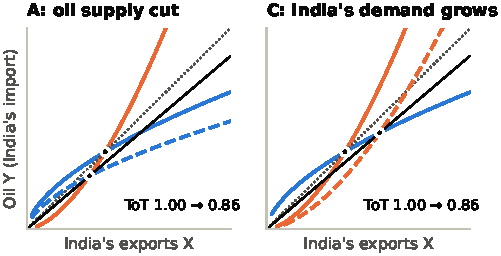
\includegraphics[width=\linewidth]{figures/offer_curves}\\[1pt]
      {\scriptsize India's ToT is the slope of the ray through the equilibrium ($P_X/P_Y$). A flatter ray means each unit of India's exports buys less oil. Data: after the 2022 shock, India's merchandise ToT fell 24\% (FY2020-21 to FY2022-23).}
    \column{.39\textwidth}
      \begin{card}\small\textbf{A supply cut works like a tariff}\\{\scriptsize OPEC+ offers less oil per unit of India's exports: its ToT improves, India's falls (L22).\par}\end{card}
      \begin{card}\small\textbf{India is not a price-taker}\\{\scriptsize As the 3rd-largest buyer, India's own demand growth also worsens its ToT (L11).\par}\end{card}
      \begin{card}\small\textbf{World booms shift both curves}\\{\scriptsize India's export demand rises too, so the sign is an empirical question: H3.\par}\end{card}
  \end{columns}
  \src{Illustrative offer curves (method of L22); ToT change from RBI Handbook Table 121 (chain-linked); EIA.}
  \note{P1 (1.5 min). This is lecture 22 applied to India. India exports a composite good X and imports oil Y; each offer curve bends towards its import axis, and India's terms of trade is the slope of the ray through the crossing point. Left: an OPEC+ cut or a war means the rest of the world offers less oil for each unit of our exports. It is the lecture's tariff case with the oil exporter doing the restricting, so its terms of trade improve and India's ray flattens, from 1.00 to 0.86 in this picture. The data agree: after the 2022 shock our merchandise terms of trade fell 24 percent. Right: India is the third-largest oil consumer, so when our own demand grows our curve shifts out and our terms of trade worsen. That is why we cannot treat India as a pure price-taker, and why we later use shocks India cannot cause. A world boom shifts both curves, so theory alone cannot sign it. That is H3. Over to P2.}
\end{frame}

% ===================================================================== P2
\begin{frame}{How big should the hit be?}
  \begin{darkcard}
    \centering $d\ln ToT \;\approx\; (s_x - s_m)\cdot d\ln P_{oil}$\qquad{\small\color{white!75!navy} oil's share in exports minus its share in imports}
  \end{darkcard}
  \vspace{4mm}
  \begin{columns}[T,onlytextwidth]
    \column{.5\textwidth}
      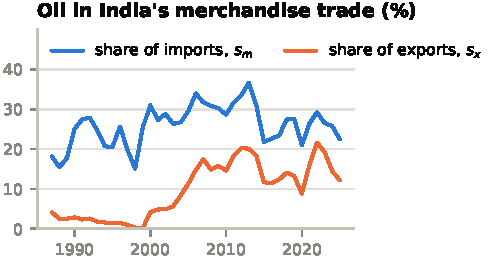
\includegraphics[width=\linewidth]{figures/oil_shares}
    \column{.47\textwidth}
      \begin{card}\stat{$-0.25 \to -0.10$}{Benchmark $s_x-s_m$, FY1999-00 to FY2025-26: net oil exposure more than halved}\end{card}
      \begin{card}\stat{$0.06 \to 4.37$}{Revealed comparative advantage in refined petroleum, 1999 to 2025 (Balassa, L08)}\end{card}
      \begin{card}\stat{0.55 vs 0.10}{Grubel--Lloyd for oil, aggregated vs crude and products separately (L17, L19)}\end{card}
  \end{columns}
  \src{RBI Handbook 2025-26 (Table 111); UNCTADstat (RCA); UN Comtrade (HS 2709, 2710).}
  \note{P2 (1 min). Before any regression, the definition of the terms of trade already tells us roughly how big the effect should be: oil's share in exports minus its share in imports, times the change in the oil price. Oil is about a quarter of India's imports, but since the Jamnagar refineries around 2000 it has also become between 9 and 22 percent of our exports. So the predicted elasticity has gone from minus 0.25 to about minus 0.10. Two lecture measures explain why. India's revealed comparative advantage in refined petroleum rose from 0.06 in 1999 to above 4: an acquired advantage built on refining scale. And the Grubel-Lloyd index of oil trade is 0.55 when crude and products are lumped together but only 0.10 when they are separated: we import crude and export fuels, which is vertical, value-adding trade. That is India's natural hedge.}
\end{frame}

% -------------------------------------------------------------- literature
\begin{frame}{What we know, and the gap}
  \begin{columns}[T,onlytextwidth]
    \column{.24\textwidth}\begin{card}[equal height group=lit]\small\textbf{Why ToT matter}\\[2pt]\scriptsize Harberger (1950); Laursen \& Metzler (1950): a worse ToT lowers real income and the trade balance.\\[2pt] How much is debated: Mendoza (1995) vs Schmitt-Groh\'e \& Uribe (2018).\end{card}
    \column{.24\textwidth}\begin{card}[equal height group=lit]\small\textbf{Oil drives ToT}\\[2pt]\scriptsize Backus \& Crucini (2000): oil explains much of the variation in ToT.\\[2pt] Kilian, Rebucci \& Spatafora (2009): the effect depends on the kind of oil shock.\end{card}
    \column{.24\textwidth}\begin{card}[equal height group=lit]\small\textbf{Shocks differ}\\[2pt]\scriptsize Hamilton (1983, 2003); Mork (1989): asymmetry.\\[2pt] Kilian (2009); Baumeister \& Hamilton (2019); K\"anzig (2021): supply vs demand.\end{card}
    \column{.24\textwidth}\begin{card}[equal height group=lit]\small\textbf{India}\\[2pt]\scriptsize Bhanumurthy, Das \& Bose (2012); Ghosh (2011); Tiwari \& Olayeni (2013); Deheri \& Sahu (2024).\\[2pt] Focus: trade balance, inflation, the rupee.\end{card}
  \end{columns}
  \vspace{1mm}
  \begin{darkcard}\small{\color{oil!60!white}\textbf{Gap.}} Indian studies model the trade balance, inflation or the rupee. We found none that models India's terms of trade directly, with a theory benchmark, identified supply and demand shocks, and the 2022 and 2026 episodes.\end{darkcard}
  \src{All references checked against Crossref/RePEc; full list in docs/references.md.}
  \note{P2 (1 min). Four strands. Why the terms of trade matter: Harberger and Laursen-Metzler show a worse terms of trade lowers real income and the trade balance; how much they drive business cycles is debated, Mendoza says a lot, Schmitt-Grohe and Uribe find under 10 percent. Our anchor paper is Backus and Crucini (2000): oil explains much of the terms-of-trade variation of industrial countries. Kilian, Rebucci and Spatafora show the external-balance effect depends on the kind of oil shock. On defining shocks: Hamilton and Mork on asymmetry, and Kilian, Baumeister-Hamilton and Kanzig on separating supply from demand. Indian work looks at the trade balance, inflation and the rupee. So our gap is the terms of trade itself, with a theory benchmark, identified shocks and the latest episodes.}
\end{frame}

% -------------------------------------------------------------- data
\begin{frame}{Data: official sources, checked line by line}
  \begin{columns}[T,onlytextwidth]
    \column{.46\textwidth}
      \small\textbf{Official agencies and published replication data only}\\[3pt]
      \begin{columns}[T,onlytextwidth]
        \column{.5\linewidth}\scriptsize
          RBI Handbook 2025-26\\ DGCI\&S trade indices\\ PPAC (Indian basket)\\ World Bank Pink Sheet\\ World Bank WDI
        \column{.5\linewidth}\scriptsize
          UNCTADstat\\ UN Comtrade\\ US EIA \quad BIS\\ Baumeister--Hamilton\\ K\"anzig (AER data)
      \end{columns}
      \vspace{5pt}
      \begin{card}\scriptsize
        \textbf{Monthly:} Apr 2019--Jun 2026 (87 months)\\
        \textbf{Annual:} FY1970-71 to FY2025-26\\
        \textbf{Merchandise ToT:} FY1994-95 to FY2025-26
      \end{card}
    \column{.51\textwidth}
      \begin{darkcard}
        {\color{oil!60!white}\large\bfseries 0 failed checks}\\
        {\scriptsize\color{white!75!navy} recomputed indices, cross-source comparisons, fiscal-year alignment}\\[3pt]
        \small\textbf{Problems we found in official tables}
        \begin{darklist}\scriptsize
          \item RBI's base-year ToT series contradict each other: $+21.7\%$ vs $-21.0\%$ (1999--2007)
          \item RBI Table 32 repeats the 2000--07 rows for 1990--97
          \item DGCI\&S export volume index jumps between 54 and 2001, so we use price indices only
          \item Three published RBI ToT values disagree with RBI's own indices
        \end{darklist}
      \end{darkcard}
  \end{columns}
  \src{data/SOURCES.md (URLs, checksums); data/validation\_report.md (all checks).}
  \note{P2 (1.5 min). Our data come only from official agencies and from the published data of peer-reviewed papers: the RBI Handbook, DGCI\&S trade indices, PPAC, the World Bank, UNCTAD, UN Comtrade, the US EIA, the BIS, and the Baumeister-Hamilton and Kanzig shock series. Every file is logged with its web address and a checksum, and a validation script runs all the cross-checks: none fails. Checking mattered. RBI's three base-year series of the terms of trade move in opposite directions over 1999 to 2007; RBI's crude-import table repeats the 2000-07 rows for 1990-97; the DGCI\&S export volume index jumps between 54 and 2001; and three published RBI values disagree with RBI's own indices. We documented and corrected each one. Over to P3.}
\end{frame}

% ===================================================================== P3
\begin{frame}{Method in four steps}
  \begin{columns}[T,onlytextwidth]
    \column{.24\textwidth}\begin{card}[height=5.1cm]\badge{1}\\[3pt]\small\textbf{Unit-root tests}\\[2pt]\footnotesize ADF, Phillips--Perron, KPSS, Zivot--Andrews\\[4pt]{\color{muted}All series stationary in differences, none I(2), so ARDL is valid}\end{card}
    \column{.24\textwidth}\begin{card}[height=5.1cm]\badge{2}\\[3pt]\small\textbf{ARDL bounds test}\\[2pt]\footnotesize H1: short-run vs long-run effect, speed of adjustment\\[4pt]{\color{muted}Works with mixed I(0)/I(1) and 54 years; short vs long run as in L13}\end{card}
    \column{.24\textwidth}\begin{card}[height=5.1cm]\badge{3}\\[3pt]\small\textbf{Nonlinear ARDL}\\[2pt]\footnotesize H2: separate effects of oil price rises and falls\\[4pt]{\color{muted}Wald tests of long-run and short-run symmetry}\end{card}
    \column{.24\textwidth}\begin{card}[height=5.1cm,colback=cardwarm,colframe=cardwarm]\badge{4}\\[3pt]\small\textbf{Shock split + local projections}\\[2pt]\footnotesize H3: supply- vs demand-driven oil prices; monthly timing\\[4pt]{\color{muted}Baumeister--Hamilton and K\"anzig shocks are not caused by India}\end{card}
  \end{columns}
  \src{Pesaran, Shin \& Smith (2001); Kripfganz \& Schneider (2020); Shin, Yu \& Greenwood-Nimmo (2014); Jord\`a (2005).}
  \note{P3 (1 min). Four steps. First, unit-root tests, including Zivot-Andrews with a break. Every series is stationary in first differences and none is I(2), so ARDL is valid. Second, the ARDL bounds test of Pesaran, Shin and Smith for H1. It handles a mix of I(0) and I(1) variables, works with our 54 years, and separates the short run from the long run, like the time horizons of lecture 13. We use finite-sample critical values. Third, the nonlinear ARDL, which splits oil prices into rises and falls, for H2. Fourth, for H3 we split each oil price change into a supply-driven and a demand-driven part using Baumeister-Hamilton's shocks, and we trace monthly timing with local projections. These shocks come from the world oil market and OPEC announcements, so India's own demand cannot cause them.}
\end{frame}

% -------------------------------------------------------------- H1
\begin{frame}{H1: oil hurts India's terms of trade, and fast}
  \begin{columns}[T,onlytextwidth]
    \column{.52\textwidth}
      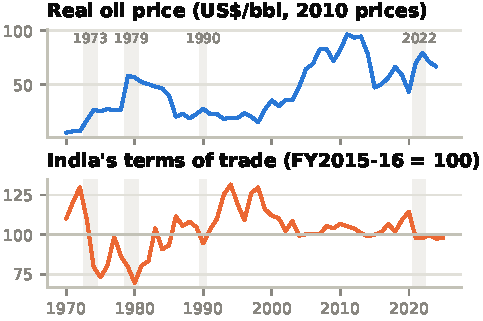
\includegraphics[width=\linewidth]{figures/oil_and_tot}
    \column{.45\textwidth}
      \begin{card}[colback=cardwarm,colframe=cardwarm]\stat{$-0.24$}{Short-run elasticity: a 10\% oil rise cuts ToT by 2.4\% the same year ($p<0.001$, robust s.e.)}\end{card}
      \begin{card}\stat{31\% a year}{of any gap closes each year (error correction $\alpha=-0.31$): the hit is large but temporary}\end{card}
      \begin{card}\stat{$-0.09$}{Long-run elasticity, not significant; bounds $F=4.74$ ($p=0.07$)}\end{card}
      {\tiny\color{muted} $-0.19$ to $-0.28$ in six specifications; diagnostics pass; CUSUM stable.}
  \end{columns}
  \src{Authors' ARDL estimates, FY1970-71 to FY2024-25 ($N=54$); World Bank WDI and Pink Sheet.}
  \note{P3 (1.5 min). The charts cover 55 years: every big oil spike, 1973, 1979, 1990, 2022, lines up with a fall in India's terms of trade. The ARDL confirms H1. The short-run elasticity is minus 0.24: a 10 percent rise in the real oil price cuts the terms of trade by 2.4 percent in the same year, significant well below 1 percent even with robust standard errors. The error-correction coefficient is minus 0.31, so about 31 percent of any deviation closes each year. The long-run elasticity is small, minus 0.09, and not significant; the bounds F of 4.74 rejects no relationship only at 10 percent against the upper bound. So oil moves our terms of trade strongly but temporarily. The short-run effect holds in all six specifications. Diagnostics: no serial correlation, normal errors, correct functional form, stable CUSUM; Breusch-Pagan found heteroskedasticity, so we report robust standard errors.}
\end{frame}

% -------------------------------------------------------------- dynamics
\begin{frame}{The hit arrives within two to three months}
  \begin{columns}[T,onlytextwidth]
    \column{.52\textwidth}
      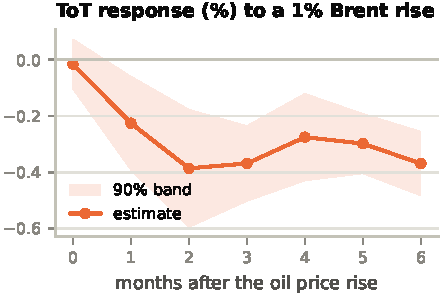
\includegraphics[width=\linewidth]{figures/local_projections}
    \column{.45\textwidth}
      \begin{card}[colback=cardwarm,colframe=cardwarm]\stat{$-0.39$}{Elasticity two months after an oil rise; almost nothing in month 0 (monthly data, Apr 2019--Jun 2026)}\end{card}
      \begin{card}\stat{1.70}{Benchmark test: theory predicts a coefficient of 1 on $(s_x-s_m)\,\Delta\ln P_{oil}$; 1 is not rejected at 5\% ($p=0.07$)}\end{card}
      \begin{card}\stat{+18\% vs +16\%}{2026 so far: export prices rose as fast as import prices (Feb--Apr), so ToT has not clearly fallen yet}\end{card}
  \end{columns}
  \src{Authors' local projections (Jord\`a 2005); DGCI\&S monthly ToT (base 2012-13); World Bank Pink Sheet; RBI Table 111.}
  \note{P3 (1.5 min). How fast does it happen? With monthly DGCI\&S data we run local projections. In the month of the price change almost nothing happens; after one to three months the terms of trade fall by about 0.2 to 0.4 percent per 1 percent oil rise, and the effect stays. The lag fits how crude is bought: cargoes are priced on earlier benchmarks and recorded at customs when they arrive. Is the size what theory predicts? Our benchmark test regresses the change in the terms of trade on the share-weighted oil change; theory says the coefficient is 1. We get 1.70 and cannot reject 1 at 5 percent. The extra comes from indirect channels like fertiliser, petrochemicals and freight. And 2026 shows the hedge working: from February to April our export unit values rose 18 percent, as fast as import unit values, so up to June the terms of trade had not clearly fallen. Single months are noisy, so we judge episodes on averages, never on one month. P4 now covers H2, H3 and policy.}
\end{frame}

% ===================================================================== P4
\begin{frame}{Symmetric, and half as large as before}
  \begin{columns}[T,onlytextwidth]
    \column{.52\textwidth}
      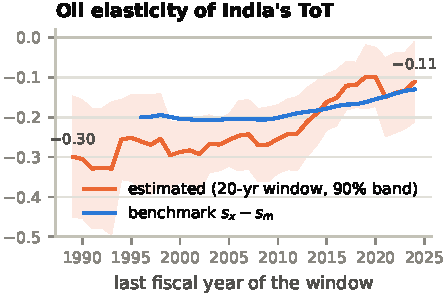
\includegraphics[width=\linewidth]{figures/rolling_elasticity}
    \column{.45\textwidth}
      \begin{card}\small\textbf{\color{oil}H2 not supported}\\[1pt]\footnotesize Short run: rise $-0.27$, fall $-0.22$; symmetry never rejected ($p=0.54$--$0.91$). A long-run asymmetry appears only with the 1970s in the sample ($p=0.28$ from 1980).\end{card}
      \begin{card}\small\textbf{\color{oil}Exposure halved}\\[1pt]\footnotesize Elasticity $-0.30$ (window to 1989) to $-0.11$ (to 2024). It tracks the benchmark ($-0.25\to-0.10$) as refined-fuel exports grew: the refining advantage works as a hedge (RCA $\approx$ 4).\end{card}
  \end{columns}
  \src{Authors' NARDL and rolling-regression estimates; WDI, Pink Sheet, RBI Table 111, UNCTADstat.}
  \note{P4 (1.2 min). H2 asked whether rises and falls have unequal effects. In the short run, clearly not: minus 0.27 for a rise, minus 0.22 for a fall, and symmetry is never rejected. The baseline long-run model finds a slightly bigger response to falls, but it disappears once we drop the 1970s and does not hold for merchandise trade. So we call the effects symmetric, and H2 is not supported: India gains from cheaper oil about as much as it loses from dearer oil. The chart shows a second and robust finding: India has become much less exposed. A 10 percent oil rise used to cut the terms of trade by about 3 percent; now it is about 1.1 percent. That matches the benchmark from P2's slide and the rise of refined-fuel exports.}
\end{frame}

% -------------------------------------------------------------- H3
\begin{frame}{H3: how much oil rises matters more than why}
  \begin{columns}[T,onlytextwidth]
    \column{.52\textwidth}
      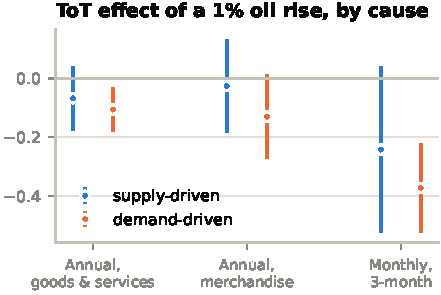
\includegraphics[width=\linewidth]{figures/supply_vs_demand}
    \column{.45\textwidth}
      \begin{card}[colback=cardwarm,colframe=cardwarm]\small\textbf{\color{oil}H3 not supported}\\[1pt]\footnotesize Demand-driven rises hurt at least as much as supply-driven ones ($p=0.53$--$0.71$ for a difference).\end{card}
      \begin{card}\small\textbf{Why}\\[1pt]\footnotesize A world boom also lifts the prices of gold, coal, fertiliser, edible oil and metals that India imports.\end{card}
      \begin{card}\small\textbf{Cross-check}\\[1pt]\footnotesize K\"anzig's OPEC-news shocks (about $+10\%$ on oil): India's ToT falls 4--5\% two to three months later.\end{card}
  \end{columns}
  \src{Authors' estimates with Baumeister \& Hamilton (2019) and K\"anzig (2021) shocks; WDI, RBI, DGCI\&S. Bars are 90\% intervals.}
  \note{P4 (1.2 min). H3 asked whether the cause matters. We split every monthly oil price change since 1975 into a supply-driven and a demand-driven part using Baumeister and Hamilton's shocks, then asked which part moves India's terms of trade. In all three samples the demand-driven part hurts at least as much, and the difference is not significant, so H3 is not supported. The offer-curve idea that a boom also raises demand for our exports does not show up, because a global boom raises the prices of everything India imports, gold, coal, fertiliser, edible oils and metals, while our manufactured exports gain less. Kanzig's OPEC announcement shocks confirm that pure supply shocks do hurt: about 4 to 5 percent after two to three months. For India, how much oil rises matters more than why.}
\end{frame}

% -------------------------------------------------------------- conclusion
\begin{frame}{What it means for India}
  \begin{columns}[T,onlytextwidth]
    \column{.44\textwidth}
      \begin{darkcard}[height=5.6cm]
        \textbf{What we found}
        \begin{darklist}\small
          \item[\color{oil}\textbf{H1}] A 10\% oil rise cuts India's ToT by 2.4\% within a year, mostly within 2--3 months
          \item[\color{oil}\textbf{H2}] Rises and falls matter about equally
          \item[\color{oil}\textbf{H3}] Demand-driven rises hurt as much as supply-driven ones
          \item[\color{oil}\textbf{+}] Exposure has halved since the 1990s: refining is India's hedge
        \end{darklist}
      \end{darkcard}
    \column{.53\textwidth}
      \small\textbf{What India can do}
      \begin{card}\scriptsize\textbf{Buffers for both directions:} strategic reserves and a fuel-tax buffer that cuts duties in spikes and rebuilds them in slumps\end{card}
      \begin{card}\scriptsize\textbf{Grow the refining hedge:} more refined and petrochemical exports raise $s_x$ (L08, L16)\end{card}
      \begin{card}\scriptsize\textbf{Diversify suppliers:} more sources weaken any one seller's market power (L16)\end{card}
      \begin{card}\scriptsize\textbf{Cut commodity dependence:} energy transition and ethanol blending, since demand booms hurt too\end{card}
  \end{columns}
  \src{Limitations (unit values are not pure prices; monthly data start in 2019; the 2026 shock is still unfolding) are in the backup slides.}
  \note{P4 (1.1 min). To sum up. H1 holds: a 10 percent oil rise cuts India's terms of trade by about 2.4 percent within a year, mostly within two to three months. H2 and H3 do not: rises and falls matter about equally, and demand-driven rises hurt as much as supply-driven ones. And our exposure has roughly halved since the 1990s because refining became an export strength. The policy lessons: because the effects are symmetric, India needs buffers that work both ways, like strategic reserves and a fuel-tax buffer; keep growing the refining hedge; diversify suppliers; and since demand booms hurt too, cut commodity-import dependence through the energy transition. Thank you, we are happy to take questions.}
\end{frame}

\begin{frame}[standout]
  Thank you\\[6pt]
  {\normalsize Questions welcome}
\end{frame}

% ===================================================================== backup
\appendix
\begin{frame}{Backup: oil episodes, fiscal-year averages}
  \centering\small\begin{tabular}{llrrrr}
\toprule
Episode & Fiscal years & Real oil & ToT (G\&S) & ToT (merch.) \\
\midrule
1973 OPEC embargo & 1972-73 to 1974-75 & +284.1\% & $-$38.6\% & -- \\
1979 Iranian revolution & 1978-79 to 1980-81 & +110.2\% & $-$19.2\% & -- \\
1990 Gulf war & 1989-90 to 1990-91 & +21.1\% & $-$9.8\% & -- \\
2008 price spike & 2006-07 to 2008-09 & +19.9\% & +4.9\% & +5.8\% \\
2014-16 price collapse & 2013-14 to 2015-16 & $-$49.9\% & $-$1.0\% & +19.4\% \\
2020 COVID crash & 2019-20 to 2020-21 & $-$26.4\% & +4.7\% & +9.6\% \\
2022 Russia-Ukraine & 2020-21 to 2022-23 & +82.8\% & $-$14.4\% & $-$23.7\% \\
\bottomrule
\end{tabular}
\\[6pt]
  \raggedright\footnotesize\color{muted} 2008 looks mild in annual averages because the spike lasted only months; the 2014--16 collapse shows the merchandise gain from cheap oil.
  \src{World Bank WDI and Pink Sheet; RBI Table 121 (chain-linked).}
\end{frame}

\begin{frame}{Backup: unit-root tests (p-values)}
  \centering\scriptsize\begin{tabular}{lrrrrrrr}
\toprule
Series & ADF lvl & ADF diff & PP lvl & PP diff & KPSS lvl & ZA lvl & ZA break \\
\midrule
ln ToT goods \& services & 0.057 & 0.000 & 0.050 & 0.000 & 0.100 & 0.391 & 1985 \\
ln ToT merchandise (FY1994-) & 0.271 & 0.001 & 0.392 & 0.000 & 0.010 & 0.062 & 2011 \\
ln real oil price & 0.053 & 0.000 & 0.050 & 0.000 & 0.013 & 0.533 & 1999 \\
ln real non-energy prices & 0.355 & 0.000 & 0.395 & 0.000 & 0.100 & 0.911 & 2005 \\
ln real gold price & 0.945 & 0.000 & 0.582 & 0.000 & 0.010 & 0.942 & 2006 \\
\bottomrule
\end{tabular}
\\[6pt]
  \raggedright\footnotesize\color{muted} ADF and PP: null of a unit root. KPSS: null of stationarity. ZA: unit root with one break. Every series is stationary in differences, so none is I(2).
  \src{Authors' tests, notebook 03.}
\end{frame}

\begin{frame}{Backup: ARDL main estimates}
  \centering\small\begin{tabular}{lrrr}
\toprule
 & Estimate & Std. error & p-value \\
\midrule
Short-run oil elasticity (same year) & $-$0.241 & 0.049 & 0.000 \\
Long-run oil elasticity & $-$0.092 & 0.059 & 0.119 \\
Long-run non-oil commodity elasticity & $-$0.249 & 0.177 & 0.159 \\
Error-correction speed $\alpha$ & $-$0.308 & 0.086 & 0.001 \\
\bottomrule
\end{tabular}
\\[6pt]
  \raggedright\footnotesize\color{muted} Bounds $F=4.74$, $p=0.025$ against I(0) and $0.070$ against I(1). Diagnostics ($p$): Breusch--Godfrey 0.90, Breusch--Pagan 0.019 (so HC1 robust s.e.: 0.040 for the short-run effect), Jarque--Bera 0.25, RESET 0.84; CUSUM and CUSUMSQ inside 5\% bands.
  \src{ARDL(1,1,1), FY1970-71 to FY2024-25, $N=54$; long-run s.e. by the delta method.}
\end{frame}

\begin{frame}{Backup: ARDL robustness}
  \centering\scriptsize\begin{tabular}{lrrrrrrr}
\toprule
Specification & N & SR oil & t & LR oil & ECT $\alpha$ & F & p (I(1)) \\
\midrule
Baseline: oil + non-oil (G\&S ToT) & 54 & $-$0.241 & $-$4.931 & $-$0.092 & $-$0.308 & 4.743 & 0.070 \\
Oil only & 54 & $-$0.195 & $-$4.577 & $-$0.084 & $-$0.241 & 4.064 & 0.173 \\
Oil + non-oil + gold & 54 & $-$0.217 & $-$4.738 & $-$0.061 & $-$0.310 & 3.538 & 0.149 \\
Brent instead of average crude & 54 & $-$0.236 & $-$4.972 & $-$0.089 & $-$0.307 & 4.709 & 0.072 \\
Post-1980 sample & 44 & $-$0.211 & $-$4.965 & $-$0.192 & $-$0.355 & 3.651 & 0.172 \\
Merchandise ToT, FY1994-2024 & 30 & $-$0.277 & $-$3.457 & $-$0.146 & $-$0.368 & 2.084 & 0.506 \\
\bottomrule
\end{tabular}

  \src{Authors' estimates, notebook 03.}
\end{frame}

\begin{frame}{Backup: NARDL symmetry tests}
  \centering\scriptsize\begin{tabular}{lrrrrrrr}
\toprule
Specification & N & $L^{+}$ & $L^{-}$ & p (LR) & $\pi^{+}$ & $\pi^{-}$ & p (SR) \\
\midrule
Baseline FY1970-2024, with non-oil control & 54 & $-$0.162 & $-$0.228 & 0.035 & $-$0.271 & $-$0.215 & 0.620 \\
No control & 54 & $-$0.199 & $-$0.285 & 0.017 & $-$0.233 & $-$0.192 & 0.735 \\
Brent & 54 & $-$0.157 & $-$0.221 & 0.036 & $-$0.261 & $-$0.217 & 0.693 \\
Extra lag of $\Delta$ToT & 53 & $-$0.119 & $-$0.180 & 0.051 & $-$0.239 & $-$0.215 & 0.831 \\
FY1975-2024 & 49 & $-$0.106 & $-$0.161 & 0.077 & $-$0.217 & $-$0.204 & 0.913 \\
FY1980-2024 (drops the 1970s shocks) & 44 & $-$0.114 & $-$0.145 & 0.275 & $-$0.245 & $-$0.172 & 0.537 \\
Merchandise ToT FY1994-2024 & 30 & $-$0.187 & $-$0.075 & 0.131 & $-$0.234 & $-$0.308 & 0.746 \\
\bottomrule
\end{tabular}
\\[6pt]
  \raggedright\footnotesize\color{muted} $L^{\pm}$: long-run effects of rises and falls; $\pi^{\pm}$: short-run. Short-run symmetry is never rejected; the long-run asymmetry needs the 1970s.
  \src{NARDL(1,1) estimates, notebook 04.}
\end{frame}

\begin{frame}{Backup: supply- vs demand-driven oil prices}
  \centering\resizebox{\linewidth}{!}{\begin{tabular}{lrrrrrr}
\toprule
Sample & N & Supply & s.e. & Demand & s.e. & p (equal) \\
\midrule
Annual G\&S ToT, FY1975-2025 & 51 & $-$0.068 & 0.066 & $-$0.106 & 0.045 & 0.707 \\
Annual merchandise ToT, FY1995-2024 & 31 & $-$0.027 & 0.097 & $-$0.130 & 0.086 & 0.547 \\
Monthly merchandise ToT, 3-month cumulative, 2019-26 & 82 & $-$0.242 & 0.172 & $-$0.373 & 0.093 & 0.535 \\
\bottomrule
\end{tabular}
}\\[6pt]
  \raggedright\footnotesize\color{muted} Supply part = fitted contribution of Baumeister--Hamilton supply shocks to the oil price change; demand part = activity, consumption and inventory shocks. K\"anzig news shock: annual $-0.95\%$ per shock (s.e.\ 0.49); monthly $-4.2\%$ and $-4.7\%$ at 2 and 3 months.
  \src{Notebook 06.}
\end{frame}

\begin{frame}{Backup: the refining hedge in trade-theory terms}
  \centering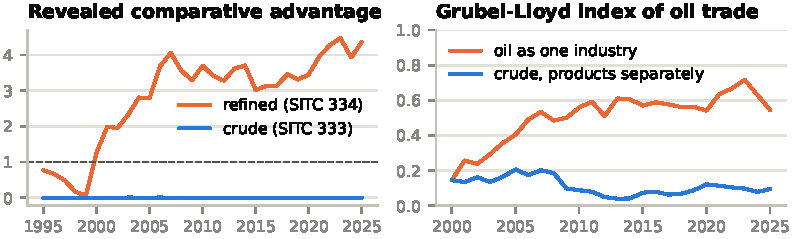
\includegraphics[height=3.7cm]{figures/rca_and_gl}\\[2pt]
  \begin{columns}[T,onlytextwidth]
    \column{.52\textwidth}\centering\resizebox{\linewidth}{!}{\begin{tabular}{lrrr}
\toprule
Year & Crude import (US\$/t) & Refined export (US\$/t) & Ratio \\
\midrule
2005 & 361.40 & 462.95 & 1.28 \\
2015 & 368.81 & 520.32 & 1.41 \\
2022 & 713.15 & 996.29 & 1.40 \\
2024 & 585.45 & 721.25 & 1.23 \\
2025 & 528.03 & 672.85 & 1.27 \\
\bottomrule
\end{tabular}
}
    \column{.44\textwidth}\scriptsize\color{muted}
      Refined exports are worth 1.13--1.41 times crude imports per tonne (2000--2025), outside the $\pm15\%$
      band that L20 uses for horizontal trade in every year except 2011 and 2012. So this is vertical, value-adding trade: India imports crude and sells refined fuel.
  \end{columns}
  \src{UNCTADstat; UN Comtrade.}
\end{frame}

\begin{frame}{Backup: monthly terms of trade, 2019--2026}
  \centering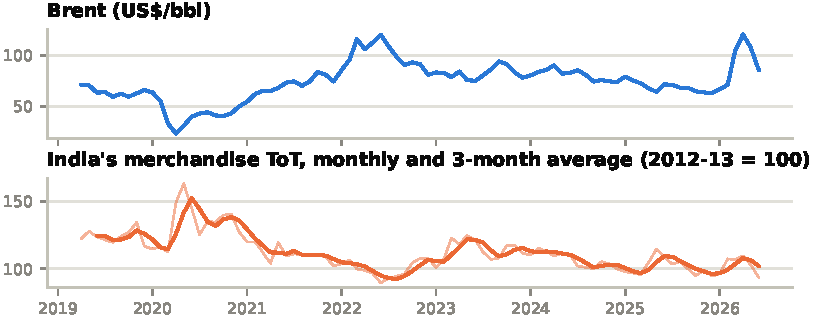
\includegraphics[width=.95\linewidth]{figures/monthly_tot}
  \src{DGCI\&S (base 2012-13); World Bank Pink Sheet.}
\end{frame}

\begin{frame}{Backup: limitations and the data fixes we made}
  \begin{itemize}\small
    \item Unit value indices are not pure price indices: they mix composition and quality changes
    \item Monthly DGCI\&S data start in April 2019; earlier monthly series are not published online
    \item DGCI\&S's two monthly bases (2012-13 and 2022-23) disagree month to month, so no episode is judged on a single month
    \item The goods-and-services ToT includes services (software), which dilutes the oil effect
    \item Imports are valued CIF and exports FOB, so freight and insurance spikes also move measured ToT (L14)
    \item Fixes: RBI base-year series linked at overlaps; NTT recomputed from the price indices; duplicated RBI rows dropped; WDI 1960s deflators excluded; mis-served PPAC file set aside
    \item The 2026 Hormuz shock is still unfolding (ToT data to June 2026)
  \end{itemize}
  \src{docs/03\_data.md; data/validation\_report.md.}
\end{frame}

\end{document}
